% REV01 Wed 23 Jun 2021 06:54:08 WIB
% START Tue 04 May 2021 13:55:16 WIB

\chapter{STRONG OF PURPOSE}

The sexton-task of piling earth above John Harmon all night long, was
not conducive to sound sleep; but Rokesmith had some broken morning
rest, and rose strengthened in his purpose. It was all over now. No
ghost should trouble Mr and Mrs Boffin’s peace; invisible and voiceless,
the ghost should look on for a little while longer at the state of
existence out of which it had departed, and then should for ever cease
to haunt the scenes in which it had no place.

He went over it all again. He had lapsed into the condition in which
he found himself, as many a man lapses into many a condition, without
perceiving the accumulative power of its separate circumstances. When
in the distrust engendered by his wretched childhood and the action for
evil--never yet for good within his knowledge then--of his father and
his father’s wealth on all within their influence, he conceived the idea
of his first deception, it was meant to be harmless, it was to last
but a few hours or days, it was to involve in it only the girl so
capriciously forced upon him and upon whom he was so capriciously
forced, and it was honestly meant well towards her. For, if he had
found her unhappy in the prospect of that marriage (through her heart
inclining to another man or for any other cause), he would seriously
have said: ‘This is another of the old perverted uses of the
misery-making money. I will let it go to my and my sister’s only
protectors and friends.’ When the snare into which he fell so
outstripped his first intention as that he found himself placarded by
the police authorities upon the London walls for dead, he confusedly
accepted the aid that fell upon him, without considering how firmly it
must seem to fix the Boffins in their accession to the fortune. When he
saw them, and knew them, and even from his vantage-ground of inspection
could find no flaw in them, he asked himself, ‘And shall I come to life
to dispossess such people as these?’ There was no good to set against
the putting of them to that hard proof. He had heard from Bella’s own
lips when he stood tapping at the door on that night of his taking
the lodgings, that the marriage would have been on her part thoroughly
mercenary. He had since tried her, in his own unknown person and
supposed station, and she not only rejected his advances but resented
them. Was it for him to have the shame of buying her, or the meanness of
punishing her? Yet, by coming to life and accepting the condition of the
inheritance, he must do the former; and by coming to life and rejecting
it, he must do the latter.

Another consequence that he had never foreshadowed, was the implication
of an innocent man in his supposed murder. He would obtain complete
retraction from the accuser, and set the wrong right; but clearly the
wrong could never have been done if he had never planned a deception.
Then, whatever inconvenience or distress of mind the deception cost him,
it was manful repentantly to accept as among its consequences, and make
no complaint.

Thus John Rokesmith in the morning, and it buried John Harmon still many
fathoms deeper than he had been buried in the night.

Going out earlier than he was accustomed to do, he encountered the
cherub at the door. The cherub’s way was for a certain space his way,
and they walked together.

It was impossible not to notice the change in the cherub’s appearance.
The cherub felt very conscious of it, and modestly remarked:

‘A present from my daughter Bella, Mr Rokesmith.’

The words gave the Secretary a stroke of pleasure, for he remembered the
fifty pounds, and he still loved the girl. No doubt it was very weak--it
always IS very weak, some authorities hold--but he loved the girl.

‘I don’t know whether you happen to have read many books of African
Travel, Mr Rokesmith?’ said R. W.

‘I have read several.’

‘Well, you know, there’s usually a King George, or a King Boy, or a King
Sambo, or a King Bill, or Bull, or Rum, or Junk, or whatever name the
sailors may have happened to give him.’

‘Where?’ asked Rokesmith.

‘Anywhere. Anywhere in Africa, I mean. Pretty well everywhere, I may
say; for black kings are cheap--and I think’--said R. W., with an
apologetic air, ‘nasty’.

‘I am much of your opinion, Mr Wilfer. You were going to say--?’

‘I was going to say, the king is generally dressed in a London hat only,
or a Manchester pair of braces, or one epaulette, or an uniform coat
with his legs in the sleeves, or something of that kind.’

‘Just so,’ said the Secretary.

‘In confidence, I assure you, Mr Rokesmith,’ observed the cheerful
cherub, ‘that when more of my family were at home and to be provided
for, I used to remind myself immensely of that king. You have no idea,
as a single man, of the difficulty I have had in wearing more than one
good article at a time.’

‘I can easily believe it, Mr Wilfer.’

‘I only mention it,’ said R. W. in the warmth of his heart, ‘as a proof
of the amiable, delicate, and considerate affection of my daughter
Bella. If she had been a little spoilt, I couldn’t have thought so very
much of it, under the circumstances. But no, not a bit. And she is so
very pretty! I hope you agree with me in finding her very pretty, Mr
Rokesmith?’

‘Certainly I do. Every one must.’

‘I hope so,’ said the cherub. ‘Indeed, I have no doubt of it. This is a
great advancement for her in life, Mr Rokesmith. A great opening of her
prospects?’

‘Miss Wilfer could have no better friends than Mr and Mrs Boffin.’

‘Impossible!’ said the gratified cherub. ‘Really I begin to think things
are very well as they are. If Mr John Harmon had lived--’

‘He is better dead,’ said the Secretary.

‘No, I won’t go so far as to say that,’ urged the cherub, a little
remonstrant against the very decisive and unpitying tone; ‘but he
mightn’t have suited Bella, or Bella mightn’t have suited him, or fifty
things, whereas now I hope she can choose for herself.’

‘Has she--as you place the confidence in me of speaking on the subject,
you will excuse my asking--has she--perhaps--chosen?’ faltered the
Secretary.

‘Oh dear no!’ returned R. W.

‘Young ladies sometimes,’ Rokesmith hinted, ‘choose without mentioning
their choice to their fathers.’

‘Not in this case, Mr Rokesmith. Between my daughter Bella and me there
is a regular league and covenant of confidence. It was ratified only the
other day. The ratification dates from--these,’ said the cherub,
giving a little pull at the lappels of his coat and the pockets of his
trousers. ‘Oh no, she has not chosen. To be sure, young George Sampson,
in the days when Mr John Harmon--’

‘Who I wish had never been born!’ said the Secretary, with a gloomy
brow.

R. W. looked at him with surprise, as thinking he had contracted an
unaccountable spite against the poor deceased, and continued: ‘In the
days when Mr John Harmon was being sought out, young George Sampson
certainly was hovering about Bella, and Bella let him hover. But it
never was seriously thought of, and it’s still less than ever to be
thought of now. For Bella is ambitious, Mr Rokesmith, and I think I may
predict will marry fortune. This time, you see, she will have the person
and the property before her together, and will be able to make her
choice with her eyes open. This is my road. I am very sorry to part
company so soon. Good morning, sir!’

The Secretary pursued his way, not very much elevated in spirits by this
conversation, and, arriving at the Boffin mansion, found Betty Higden
waiting for him.

‘I should thank you kindly, sir,’ said Betty, ‘if I might make so bold
as have a word or two wi’ you.’

She should have as many words as she liked, he told her; and took her
into his room, and made her sit down.

‘’Tis concerning Sloppy, sir,’ said Betty. ‘And that’s how I come here
by myself. Not wishing him to know what I’m a-going to say to you, I got
the start of him early and walked up.’

‘You have wonderful energy,’ returned Rokesmith. ‘You are as young as I
am.’

Betty Higden gravely shook her head. ‘I am strong for my time of life,
sir, but not young, thank the Lord!’

‘Are you thankful for not being young?’

‘Yes, sir. If I was young, it would all have to be gone through again,
and the end would be a weary way off, don’t you see? But never mind me;
‘tis concerning Sloppy.’

‘And what about him, Betty?’

‘’Tis just this, sir. It can’t be reasoned out of his head by any powers
of mine but what that he can do right by your kind lady and gentleman
and do his work for me, both together. Now he can’t. To give himself up
to being put in the way of arning a good living and getting on, he must
give me up. Well; he won’t.’

‘I respect him for it,’ said Rokesmith.

‘DO ye, sir? I don’t know but what I do myself. Still that don’t make it
right to let him have his way. So as he won’t give me up, I’m a-going to
give him up.’

‘How, Betty?’

‘I’m a-going to run away from him.’

With an astonished look at the indomitable old face and the bright eyes,
the Secretary repeated, ‘Run away from him?’

‘Yes, sir,’ said Betty, with one nod. And in the nod and in the firm set
of her mouth, there was a vigour of purpose not to be doubted.

‘Come, come!’ said the Secretary. ‘We must talk about this. Let us take
our time over it, and try to get at the true sense of the case and the
true course, by degrees.’

‘Now, lookee here, by dear,’ returned old Betty--‘asking your excuse
for being so familiar, but being of a time of life a’most to be your
grandmother twice over. Now, lookee, here. ‘Tis a poor living and a
hard as is to be got out of this work that I’m a doing now, and but for
Sloppy I don’t know as I should have held to it this long. But it did
just keep us on, the two together. Now that I’m alone--with even Johnny
gone--I’d far sooner be upon my feet and tiring of myself out, than a
sitting folding and folding by the fire. And I’ll tell you why. There’s
a deadness steals over me at times, that the kind of life favours and I
don’t like. Now, I seem to have Johnny in my arms--now, his mother--now,
his mother’s mother--now, I seem to be a child myself, a lying once
again in the arms of my own mother--then I get numbed, thought and
sense, till I start out of my seat, afeerd that I’m a growing like the
poor old people that they brick up in the Unions, as you may sometimes
see when they let ‘em out of the four walls to have a warm in the sun,
crawling quite scared about the streets. I was a nimble girl, and have
always been a active body, as I told your lady, first time ever I see
her good face. I can still walk twenty mile if I am put to it. I’d far
better be a walking than a getting numbed and dreary. I’m a good fair
knitter, and can make many little things to sell. The loan from your
lady and gentleman of twenty shillings to fit out a basket with, would
be a fortune for me. Trudging round the country and tiring of myself
out, I shall keep the deadness off, and get my own bread by my own
labour. And what more can I want?’

‘And this is your plan,’ said the Secretary, ‘for running away?’

‘Show me a better! My deary, show me a better! Why, I know very well,’
said old Betty Higden, ‘and you know very well, that your lady and
gentleman would set me up like a queen for the rest of my life, if so be
that we could make it right among us to have it so. But we can’t make it
right among us to have it so. I’ve never took charity yet, nor yet has
any one belonging to me. And it would be forsaking of myself indeed, and
forsaking of my children dead and gone, and forsaking of their children
dead and gone, to set up a contradiction now at last.’

‘It might come to be justifiable and unavoidable at last,’ the Secretary
gently hinted, with a slight stress on the word.

‘I hope it never will! It ain’t that I mean to give offence by being
anyways proud,’ said the old creature simply, ‘but that I want to be of
a piece like, and helpful of myself right through to my death.’

‘And to be sure,’ added the Secretary, as a comfort for her, ‘Sloppy
will be eagerly looking forward to his opportunity of being to you what
you have been to him.’

‘Trust him for that, sir!’ said Betty, cheerfully. ‘Though he had need
to be something quick about it, for I’m a getting to be an old one. But
I’m a strong one too, and travel and weather never hurt me yet! Now, be
so kind as speak for me to your lady and gentleman, and tell ‘em what I
ask of their good friendliness to let me do, and why I ask it.’

The Secretary felt that there was no gainsaying what was urged by
this brave old heroine, and he presently repaired to Mrs Boffin and
recommended her to let Betty Higden have her way, at all events for the
time. ‘It would be far more satisfactory to your kind heart, I know,’
he said, ‘to provide for her, but it may be a duty to respect this
independent spirit.’ Mrs Boffin was not proof against the consideration
set before her. She and her husband had worked too, and had brought
their simple faith and honour clean out of dustheaps. If they owed a
duty to Betty Higden, of a surety that duty must be done.

‘But, Betty,’ said Mrs Boffin, when she accompanied John Rokesmith back
to his room, and shone upon her with the light of her radiant face,
‘granted all else, I think I wouldn’t run away’.

‘’Twould come easier to Sloppy,’ said Mrs Higden, shaking her head.
‘’Twould come easier to me too. But ‘tis as you please.’

‘When would you go?’

‘Now,’ was the bright and ready answer. ‘To-day, my deary, to-morrow.
Bless ye, I am used to it. I know many parts of the country well. When
nothing else was to be done, I have worked in many a market-garden afore
now, and in many a hop-garden too.’

‘If I give my consent to your going, Betty--which Mr Rokesmith thinks I
ought to do--’

Betty thanked him with a grateful curtsey.

‘--We must not lose sight of you. We must not let you pass out of our
knowledge. We must know all about you.’

‘Yes, my deary, but not through letter-writing, because
letter-writing--indeed, writing of most sorts hadn’t much come up for
such as me when I was young. But I shall be to and fro. No fear of
my missing a chance of giving myself a sight of your reviving face.
Besides,’ said Betty, with logical good faith, ‘I shall have a debt to
pay off, by littles, and naturally that would bring me back, if nothing
else would.’

‘MUST it be done?’ asked Mrs Boffin, still reluctant, of the Secretary.

‘I think it must.’

After more discussion it was agreed that it should be done, and Mrs
Boffin summoned Bella to note down the little purchases that were
necessary to set Betty up in trade. ‘Don’t ye be timorous for me, my
dear,’ said the stanch old heart, observant of Bella’s face: ‘when I
take my seat with my work, clean and busy and fresh, in a country
market-place, I shall turn a sixpence as sure as ever a farmer’s wife
there.’

The Secretary took that opportunity of touching on the practical
question of Mr Sloppy’s capabilities. He would have made a wonderful
cabinet-maker, said Mrs Higden, ‘if there had been the money to put him
to it.’ She had seen him handle tools that he had borrowed to mend
the mangle, or to knock a broken piece of furniture together, in a
surprising manner. As to constructing toys for the Minders, out of
nothing, he had done that daily. And once as many as a dozen people had
got together in the lane to see the neatness with which he fitted the
broken pieces of a foreign monkey’s musical instrument. ‘That’s well,’
said the Secretary. ‘It will not be hard to find a trade for him.’

John Harmon being buried under mountains now, the Secretary that very
same day set himself to finish his affairs and have done with him. He
drew up an ample declaration, to be signed by Rogue Riderhood (knowing
he could get his signature to it, by making him another and much shorter
evening call), and then considered to whom should he give the document?
To Hexam’s son, or daughter? Resolved speedily, to the daughter. But it
would be safer to avoid seeing the daughter, because the son had seen
Julius Handford, and--he could not be too careful--there might possibly
be some comparison of notes between the son and daughter, which would
awaken slumbering suspicion, and lead to consequences. ‘I might even,’
he reflected, ‘be apprehended as having been concerned in my own
murder!’ Therefore, best to send it to the daughter under cover by the
post. Pleasant Riderhood had undertaken to find out where she lived,
and it was not necessary that it should be attended by a single word of
explanation. So far, straight.

But, all that he knew of the daughter he derived from Mrs Boffin’s
accounts of what she heard from Mr Lightwood, who seemed to have a
reputation for his manner of relating a story, and to have made this
story quite his own. It interested him, and he would like to have
the means of knowing more--as, for instance, that she received the
exonerating paper, and that it satisfied her--by opening some channel
altogether independent of Lightwood: who likewise had seen Julius
Handford, who had publicly advertised for Julius Handford, and whom
of all men he, the Secretary, most avoided. ‘But with whom the common
course of things might bring me in a moment face to face, any day in the
week or any hour in the day.’

Now, to cast about for some likely means of opening such a channel. The
boy, Hexam, was training for and with a schoolmaster. The Secretary knew
it, because his sister’s share in that disposal of him seemed to be
the best part of Lightwood’s account of the family. This young fellow,
Sloppy, stood in need of some instruction. If he, the Secretary, engaged
that schoolmaster to impart it to him, the channel might be opened. The
next point was, did Mrs Boffin know the schoolmaster’s name? No, but she
knew where the school was. Quite enough. Promptly the Secretary wrote
to the master of that school, and that very evening Bradley Headstone
answered in person.

The Secretary stated to the schoolmaster how the object was, to send to
him for certain occasional evening instruction, a youth whom Mr and Mrs
Boffin wished to help to an industrious and useful place in life. The
schoolmaster was willing to undertake the charge of such a pupil. The
Secretary inquired on what terms? The schoolmaster stated on what terms.
Agreed and disposed of.

‘May I ask, sir,’ said Bradley Headstone, ‘to whose good opinion I owe a
recommendation to you?’

‘You should know that I am not the principal here. I am Mr Boffin’s
Secretary. Mr Boffin is a gentleman who inherited a property of which
you may have heard some public mention; the Harmon property.’

‘Mr Harmon,’ said Bradley: who would have been a great deal more at a
loss than he was, if he had known to whom he spoke: ‘was murdered and
found in the river.’

‘Was murdered and found in the river.’

‘It was not--’

‘No,’ interposed the Secretary, smiling, ‘it was not he who recommended
you. Mr Boffin heard of you through a certain Mr Lightwood. I think you
know Mr Lightwood, or know of him?’

‘I know as much of him as I wish to know, sir. I have no acquaintance
with Mr Lightwood, and I desire none. I have no objection to Mr
Lightwood, but I have a particular objection to some of Mr Lightwood’s
friends--in short, to one of Mr Lightwood’s friends. His great friend.’

He could hardly get the words out, even then and there, so fierce did
he grow (though keeping himself down with infinite pains of repression),
when the careless and contemptuous bearing of Eugene Wrayburn rose
before his mind.

The Secretary saw there was a strong feeling here on some sore point,
and he would have made a diversion from it, but for Bradley’s holding to
it in his cumbersome way.

‘I have no objection to mention the friend by name,’ he said, doggedly.
‘The person I object to, is Mr Eugene Wrayburn.’

The Secretary remembered him. In his disturbed recollection of that
night when he was striving against the drugged drink, there was but a
dim image of Eugene’s person; but he remembered his name, and his manner
of speaking, and how he had gone with them to view the body, and where
he had stood, and what he had said.

‘Pray, Mr Headstone, what is the name,’ he asked, again trying to make a
diversion, ‘of young Hexam’s sister?’

‘Her name is Lizzie,’ said the schoolmaster, with a strong contraction
of his whole face.

‘She is a young woman of a remarkable character; is she not?’

‘She is sufficiently remarkable to be very superior to Mr Eugene
Wrayburn--though an ordinary person might be that,’ said the
schoolmaster; ‘and I hope you will not think it impertinent in me, sir,
to ask why you put the two names together?’

‘By mere accident,’ returned the Secretary. ‘Observing that Mr Wrayburn
was a disagreeable subject with you, I tried to get away from it: though
not very successfully, it would appear.’

‘Do you know Mr Wrayburn, sir?’

‘No.’

‘Then perhaps the names cannot be put together on the authority of any
representation of his?’

‘Certainly not.’

‘I took the liberty to ask,’ said Bradley, after casting his eyes on
the ground, ‘because he is capable of making any representation, in the
swaggering levity of his insolence. I--I hope you will not misunderstand
me, sir. I--I am much interested in this brother and sister, and the
subject awakens very strong feelings within me. Very, very, strong
feelings.’ With a shaking hand, Bradley took out his handkerchief and
wiped his brow.

The Secretary thought, as he glanced at the schoolmaster’s face, that he
had opened a channel here indeed, and that it was an unexpectedly dark
and deep and stormy one, and difficult to sound. All at once, in the
midst of his turbulent emotions, Bradley stopped and seemed to challenge
his look. Much as though he suddenly asked him, ‘What do you see in me?’

‘The brother, young Hexam, was your real recommendation here,’ said the
Secretary, quietly going back to the point; ‘Mr and Mrs Boffin happening
to know, through Mr Lightwood, that he was your pupil. Anything that
I ask respecting the brother and sister, or either of them, I ask for
myself out of my own interest in the subject, and not in my official
character, or on Mr Boffin’s behalf. How I come to be interested, I need
not explain. You know the father’s connection with the discovery of Mr
Harmon’s body.’

‘Sir,’ replied Bradley, very restlessly indeed, ‘I know all the
circumstances of that case.’

‘Pray tell me, Mr Headstone,’ said the Secretary. ‘Does the sister
suffer under any stigma because of the impossible accusation--groundless
would be a better word--that was made against the father, and
substantially withdrawn?’

‘No, sir,’ returned Bradley, with a kind of anger.

‘I am very glad to hear it.’

‘The sister,’ said Bradley, separating his words over-carefully, and
speaking as if he were repeating them from a book, ‘suffers under no
reproach that repels a man of unimpeachable character who had made
for himself every step of his way in life, from placing her in his own
station. I will not say, raising her to his own station; I say, placing
her in it. The sister labours under no reproach, unless she should
unfortunately make it for herself. When such a man is not deterred from
regarding her as his equal, and when he has convinced himself that
there is no blemish on her, I think the fact must be taken to be pretty
expressive.’

‘And there is such a man?’ said the Secretary.

Bradley Headstone knotted his brows, and squared his large lower jaw,
and fixed his eyes on the ground with an air of determination that
seemed unnecessary to the occasion, as he replied: ‘And there is such a
man.’

The Secretary had no reason or excuse for prolonging the conversation,
and it ended here. Within three hours the oakum-headed apparition once
more dived into the Leaving Shop, and that night Rogue Riderhood’s
recantation lay in the post office, addressed under cover to Lizzie
Hexam at her right address.

All these proceedings occupied John Rokesmith so much, that it was not
until the following day that he saw Bella again. It seemed then to be
tacitly understood between them that they were to be as distantly easy
as they could, without attracting the attention of Mr and Mrs Boffin to
any marked change in their manner. The fitting out of old Betty Higden
was favourable to this, as keeping Bella engaged and interested, and as
occupying the general attention.

‘I think,’ said Rokesmith, when they all stood about her, while she
packed her tidy basket--except Bella, who was busily helping on her
knees at the chair on which it stood; ‘that at least you might keep a
letter in your pocket, Mrs Higden, which I would write for you and date
from here, merely stating, in the names of Mr and Mrs Boffin, that they
are your friends;--I won’t say patrons, because they wouldn’t like it.’

‘No, no, no,’ said Mr Boffin; ‘no patronizing! Let’s keep out of THAT,
whatever we come to.’

‘There’s more than enough of that about, without us; ain’t there,
Noddy?’ said Mrs Boffin.

‘I believe you, old lady!’ returned the Golden Dustman. ‘Overmuch
indeed!’

‘But people sometimes like to be patronized; don’t they, sir?’ asked
Bella, looking up.

‘I don’t. And if THEY do, my dear, they ought to learn better,’ said Mr
Boffin. ‘Patrons and Patronesses, and Vice-Patrons and Vice-Patronesses,
and Deceased Patrons and Deceased Patronesses, and Ex-Vice-Patrons and
Ex-Vice-Patronesses, what does it all mean in the books of the Charities
that come pouring in on Rokesmith as he sits among ‘em pretty well up to
his neck! If Mr Tom Noakes gives his five shillings ain’t he a Patron,
and if Mrs Jack Styles gives her five shillings ain’t she a Patroness?
What the deuce is it all about? If it ain’t stark staring impudence,
what do you call it?’

‘Don’t be warm, Noddy,’ Mrs Boffin urged.

‘Warm!’ cried Mr Boffin. ‘It’s enough to make a man smoking hot. I can’t
go anywhere without being Patronized. I don’t want to be Patronized. If
I buy a ticket for a Flower Show, or a Music Show, or any sort of Show,
and pay pretty heavy for it, why am I to be Patroned and Patronessed as
if the Patrons and Patronesses treated me? If there’s a good thing to be
done, can’t it be done on its own merits? If there’s a bad thing to
be done, can it ever be Patroned and Patronessed right? Yet when a new
Institution’s going to be built, it seems to me that the bricks and
mortar ain’t made of half so much consequence as the Patrons and
Patronesses; no, nor yet the objects. I wish somebody would tell me
whether other countries get Patronized to anything like the extent of
this one! And as to the Patrons and Patronesses themselves, I wonder
they’re not ashamed of themselves. They ain’t Pills, or Hair-Washes, or
Invigorating Nervous Essences, to be puffed in that way!’

Having delivered himself of these remarks, Mr Boffin took a trot,
according to his usual custom, and trotted back to the spot from which
he had started.

‘As to the letter, Rokesmith,’ said Mr Boffin, ‘you’re as right as a
trivet. Give her the letter, make her take the letter, put it in her
pocket by violence. She might fall sick. You know you might fall sick,’
said Mr Boffin. ‘Don’t deny it, Mrs Higden, in your obstinacy; you know
you might.’

Old Betty laughed, and said that she would take the letter and be
thankful.

‘That’s right!’ said Mr Boffin. ‘Come! That’s sensible. And don’t be
thankful to us (for we never thought of it), but to Mr Rokesmith.’

The letter was written, and read to her, and given to her.

‘Now, how do you feel?’ said Mr Boffin. ‘Do you like it?’

‘The letter, sir?’ said Betty. ‘Ay, it’s a beautiful letter!’

‘No, no, no; not the letter,’ said Mr Boffin; ‘the idea. Are you sure
you’re strong enough to carry out the idea?’

‘I shall be stronger, and keep the deadness off better, this way, than
any way left open to me, sir.’

‘Don’t say than any way left open, you know,’ urged Mr Boffin; ‘because
there are ways without end. A housekeeper would be acceptable over
yonder at the Bower, for instance. Wouldn’t you like to see the
Bower, and know a retired literary man of the name of Wegg that lives
there--WITH a wooden leg?’

Old Betty was proof even against this temptation, and fell to adjusting
her black bonnet and shawl.

‘I wouldn’t let you go, now it comes to this, after all,’ said Mr
Boffin, ‘if I didn’t hope that it may make a man and a workman of
Sloppy, in as short a time as ever a man and workman was made yet. Why,
what have you got there, Betty? Not a doll?’

It was the man in the Guards who had been on duty over Johnny’s bed.
The solitary old woman showed what it was, and put it up quietly in her
dress. Then, she gratefully took leave of Mrs Boffin, and of Mr Boffin,
and of Rokesmith, and then put her old withered arms round Bella’s young
and blooming neck, and said, repeating Johnny’s words: ‘A kiss for the
boofer lady.’

The Secretary looked on from a doorway at the boofer lady thus
encircled, and still looked on at the boofer lady standing alone there,
when the determined old figure with its steady bright eyes was trudging
through the streets, away from paralysis and pauperism.

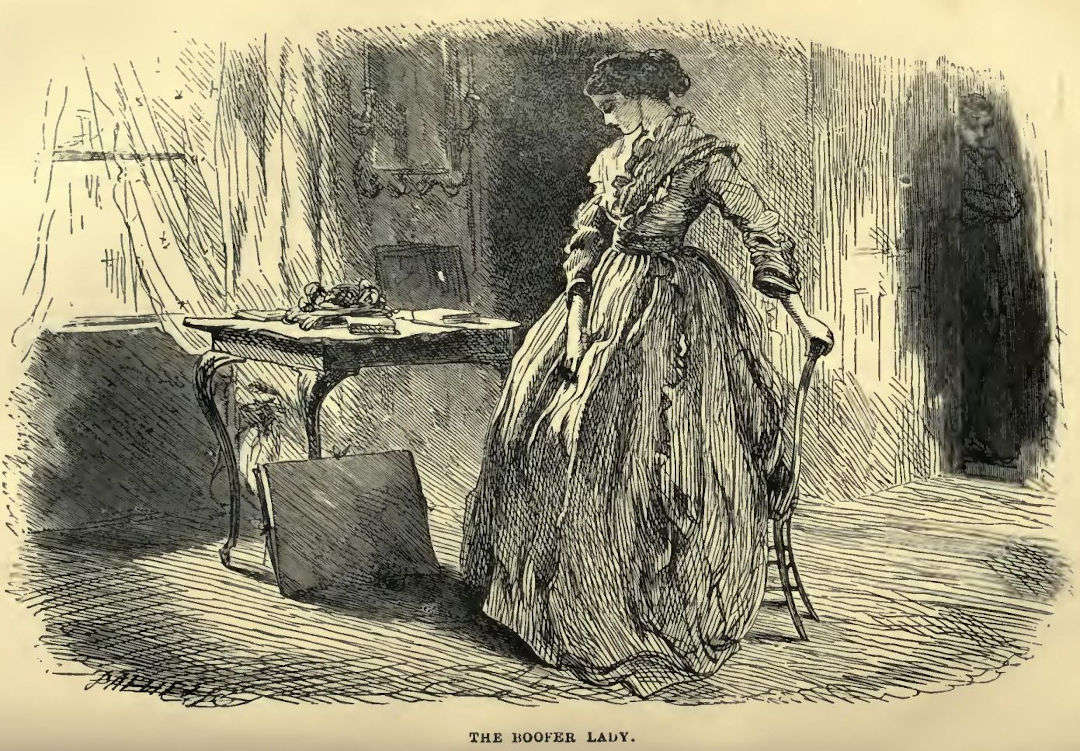
\includegraphics[scale=2.3]{02-14-01}

